\section{Parallelization}
\label{sec:par}

\newcommand{\abs}[1]{\mid \! {#1} \! \mid}

The purpose of this section is to discuss the 
\normindex{parallelization} of the 
principle MD algorithm and not to describe the algorithms that are in 
practical use for molecular systems with their complex variety of atoms 
and terms in the force field descriptions. We shall therefore consider 
as an example a simple system consisting only of a single type of atoms 
with a simple form of the interaction potential. The emphasis will be 
on the special problems that arise when the algorithm is implemented on 
a parallel computer. 

The simple model problem already contains the bottleneck of all MD 
simulations: the computationally intensive evaluation of the 
{\em non-bonded} forces between pairs of atoms, based on the distance 
between particles. Complex molecular systems will in addition 
involve many different kinds of {\em bonded} forces between designated 
atoms. Such interactions add to the complexity of the algorithm but do 
not modify the basic considerations concerning parallelization.


\subsection{Methods of parallelization}
There are a number of methods to parallelize the MD algorithm, each of
them with their own advantages and disadvantages. The method to 
choose depends on the hardware and compilers available.
We list them here:
\begin{enumerate}
\item[1]        {\em \normindex{Message Passing}.}\\
                In this method, which is more or less the traditional
                way of parallel programming, all the parallelism is
                explicitly programmed by the user. The disadvantage
                is that it takes extra code and effort, the advantage
                is that the programmer keeps full control over the data
                flow and can do optimizations a compiler could not come 
                up with. 

                The implementation is typically done by calling a set of 
                library routines to send and receive data to and from 
                other processors. Almost all hardware vendors support 
                this way of
                parallelism in their C and Fortran compilers.
                
\item[2]        {\em \swapindex{Data}{Parallel}.}\\
                This method lets the user define arrays on which to
                operate in parallel. Programming this way is much
                like vectorizing: recurrence is not parallelized
                ({\eg} {\tt for(i=1; (i<MAX); i++) a[i] = a[i-1] + 1;}
                does not vectorize and not parallelize, because for
                every i the result from the previous step is needed).

                The advantage of data parallelism is that it is
                easier for the user; the compiler takes care of the
                parallelism. The disadvantage is that it is supported
                by a small (though growing) number of hardware vendors,
                and that it is much harder to maintain a program that has to
                run on both parallel and sequential machines, because
                the only standard language that supports it is Fortran-90
                which is not available on many platforms.
\end{enumerate}
Both methods allow for the MD algorithm to be implemented without much
trouble. Message passing MD algorithms have been published
since the mid 80's (\cite{Fincham87}, \cite{Raine89}) 
and development is still continuing. 
Data parallel programming is newer,
but starting from a well vectorized program it is not hard to do.

Our implementation of MD is a message passing one, the reason for which
is partly historical: the project to develop a parallel MD program started
when Fortran-90 was still in the making, and no compilers were
expected to be available. 
At current, we still believe that message passing is the way
to go, after having done some experiments with data parallel programming on a
Connection Machine (CM-5), because of portability to other hardware,
the poor performance of the code produced by the compilers 
and because this way of programming
has the same drawback as vectorization: the part of the program that is
not vectorized or parallelized determines the runtime of the program
(\normindex{Amdahl's law}).

The approach we took to parallelism was a minimalist one: use as few
non-standard elements in the software as possible, and use the
simplest \swapindex{processor}{topology} that does the job. We therefore 
decided to use a standard language (ANSI-C) with as few non-standard
routines as possible. We only use 5 communication routines that are
non-standard. It is therefore very easy to port our code to other machines.

For an $O(N^2)$ problem like MD, one of the best schemes for the
interprocessor connections is a ring, so our software demands that a
ring is present in the interprocessor connections. A ring can essentially
always be mapped onto another network like a \normindex{hypercube}, a
bus interface (Ethernet {\eg} using 
\seeindex{Message Passing Interface}{MPI} \normindex{MPI}) or 
a \normindex{tree}
(CM-5). Some hardware vendors have very luxurious connection schemes
that connect every processor to every other processor, but we do not
really need it and so do not use it even though it might come in handy
at times. The advantage with this simple scheme is that {\gromacs}
performs extremely well even on inexpensive workstation clusters.

When using a message passing scheme one has to divide the particles 
over processors, which can be done in two ways:
\begin{itemize}
\item   {\em \swapindex{Space}{Decomposition}.}\\
        An element of space is allocated to each processor, when dividing
        a cubic box with edge $b$ over $P$ processors this can be done 
        by giving
        each processor a slab of length $b/P$. This method 
        has the advantage
        that each processor has about the same number of interactions
        to calculate (at least when the simulated system has a homogeneous
        density, like a liquid or a gas). The disadvantage is that a lot of
        bookkeeping is necessary for particles that move over processor
        boundaries. When using more complex systems, such as macromolecules there
        are also 3- and 4-atom interactions that make 
  	the bookkeeping too complicated for our taste.
\item   {\em \swapindex{Particle}{Decomposition}.}\\
        Every processor is allocated a number of particles. When
        dividing $N$ particles over $P$ processors each processor will
        get $N/P$ particles. The implementation of this method
        is described in the next section.
\end{itemize}

\begin {figure}[p]
\centerline{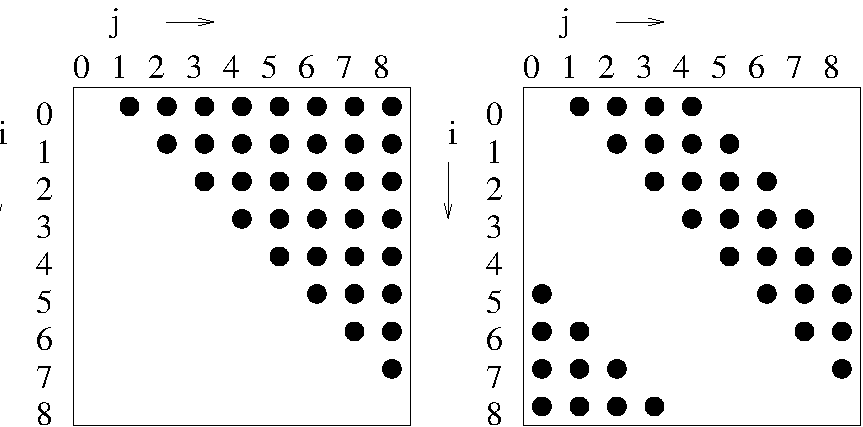
\includegraphics[width=10cm]{plots/int_mat}}
\caption[The interaction matrix.]{The interaction matrix (left) and
the same using action$~=~-$reaction (right).}
\label{fig:int_mat}
\end {figure}

\begin{table}[p]
\centerline{
\newcolumntype{s}[1]{D{/}{/}{#1}}
\begin{tabular}{|l|s4|s4|s4|s4|}
\dline
        & \mcc{1}{i mod 2 = 0}
                & \mcc{1}{i mod 2 = 0}
                                & \mcc{1}{i mod 2 = 1}
                                                & \mcc{1}{i mod 2 = 1} \\
        & \mcc{1}{i $<$ N/2} 
                & \mcc{1}{i $\ge$ N/2}
                                & \mcc{1}{i $<$ N/2}
                                                & \mcc{1}{i $\ge$ N/2} \\
\hline
N mod 2 = 1     & N/2   & N/2           & N/2           & N/2           \\
N mod 4 = 2     & N/2   & N/2           & N/2 - 1       & N/2 - 1       \\
N mod 4 = 0     & N/2   & N/2 - 1       & N/2 - 1       & N/2           \\
\dline
\end{tabular}
}
\caption[The number of interactions between particles.]{The number of
interactions between particles. The number of $j$ particles per $i$
particle is a function of the total number of particles $N$ and
particle number $i$. Note that here the $/$ operator is used for
integer division, {\ie} truncating the reminder.}
\label{tab:decomp}
\end{table}

\begin{figure}[p]
\centerline{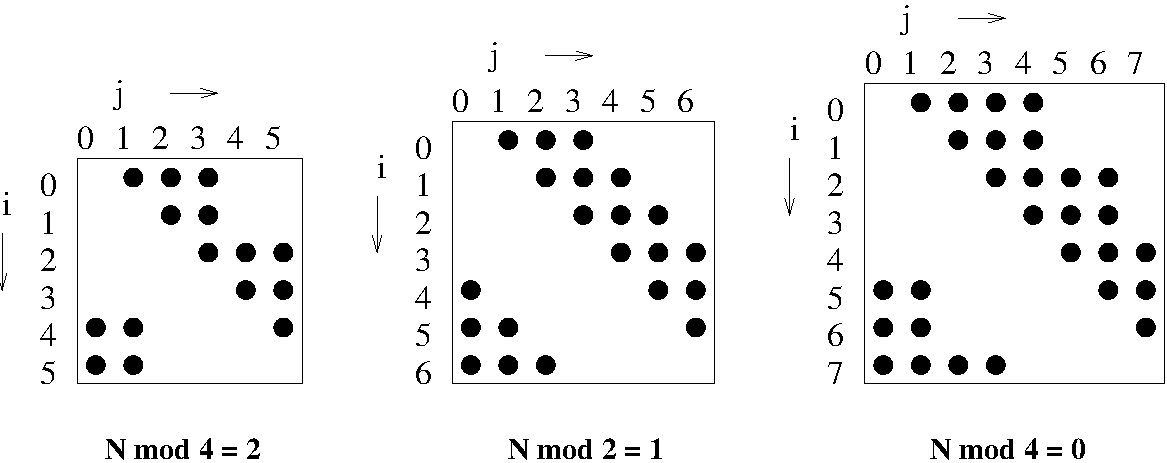
\includegraphics[width=\linewidth]{plots/decomp}}
\caption[Interaction matrices for different $N$.]{Interaction matrices for different $N$. The number of $j$-particles an $i$-particle interacts with depends on the {\em total} number of particles and on the {\em particle number}.}
\label{fig:decomp}
\end{figure}

\subsection{MD on a ring of processors}
When a neighbor list is not used the MD problem is in principle an $O(N^2)$ 
problem as each particle can interact
with every other. This can be simplified using Newton's third law
\beq
F_{ij}  ~=~     -F_{ji}
\label{eqn:Newt3}
\eeq
This implies that there is half a matrix of interactions (without diagonal, 
a particle does not interact with itself) to consider (\figref{int_mat}).
When we reflect the upper right triangle of interactions to the lower
left triangle of the matrix, we still cover all possible interactions,
but now every row in the matrix has almost the same number of points
or possible interactions.  We can now assign a (preferably equal)
number of rows to each processor to compute the forces and at the same
time a number of particles to do the update on, the {\em home}
particles. The number of interactions per particle is dependent on the
{\em total number} $N$ of particles (see \figref{decomp}) and on the
{\em particle number} $i$.  The exact formulae are given in
\tabref{decomp}.

A flow chart of the algorithm is given in \figref{mdpar}.
\begin{figure}
\centerline{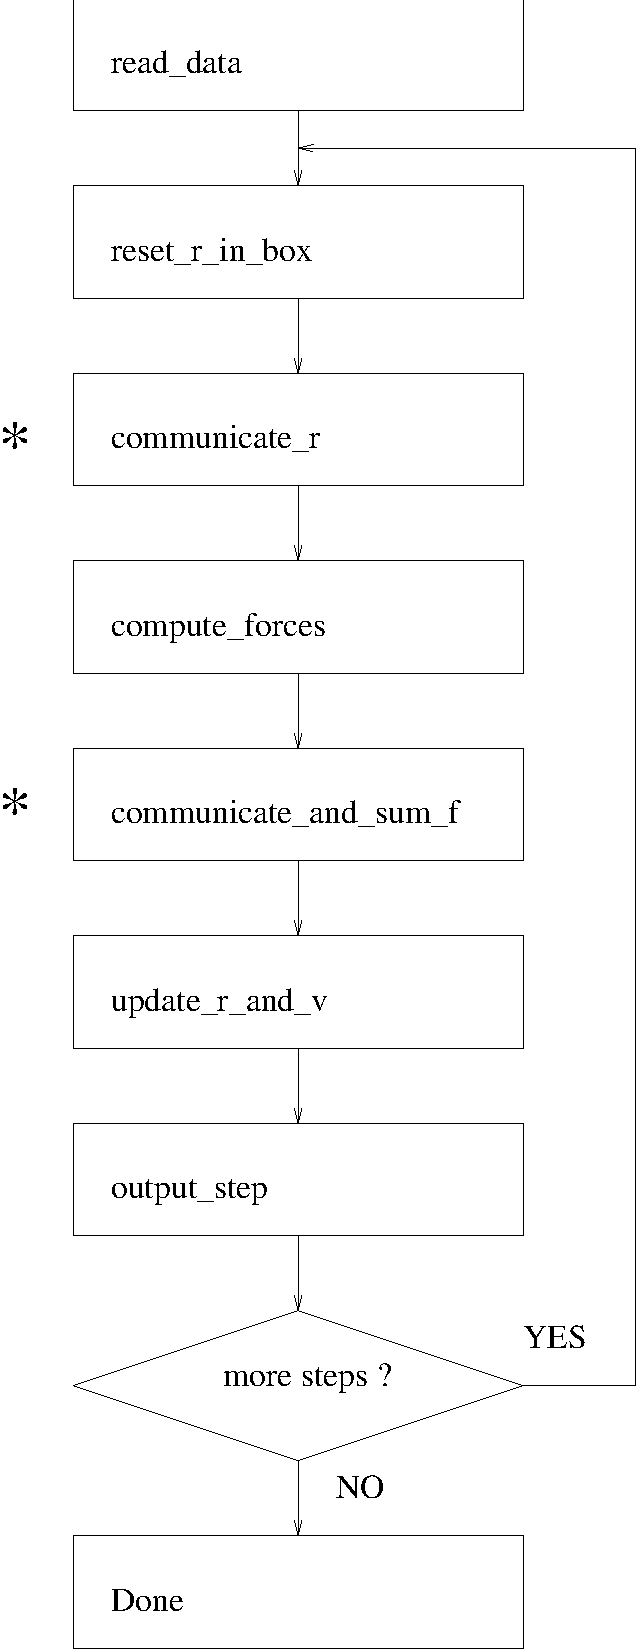
\includegraphics[height=18cm]{plots/mdpar}}
\caption[The Parallel MD algorithm.]{The Parallel MD algorithm. If
the steps marked * are left out we have the sequential algorithm
again.}
\label{fig:mdpar}
\end{figure}
\vfill

It is the same as the sequential algorithm, except for two
communication steps. After the particles have been reset in the box,
each processor sends its coordinates onward (left) and then starts computation
of the forces.  After this step each processor holds the {\em partial
forces} for the available particles, {\eg} processor 0 holds forces
acting on home particles from processor 0, 1, 2 and 3. These forces
must be accumulated and sent back (right) to the home
processor. Finally the update of the velocity and coordinates is done
on the home processor.

The {\tt communicate\_r} routine is given below in the full C-code:\\
\begin{footnotesize}
\begin{tt}
void communicate\_r(int nprocs,int pid,rvec vecs[],int start[],int homenr[])\\
/* \\
 * nprocs = number of processors\\
 * pid    = processor id (0..nprocs-1)\\
 * vecs   = vectors\\
 * start  = starting index in vecs for each processor\\
 * homenr = number of home particles for each processor\\
 */\\
{\\
  int i;        /* processor counter */\\
  int shift;    /* the amount of processors to communicate with */\\
  int cur;      /* current processor to send data from */\\
  int next;     /* next processor on a ring (using modulo) */\\
\\
  cur   = pid;\\
  shift = nprocs/2;\\
\\
  for (i=0; (i<shift); i++) {\\
    next=(cur+1) \% nprocs;     \\ 
    send   (left,  vecs[start[cur]],  homenr[cur]);\\
    receive(right, vecs[start[next]], homenr[next]);\\
    cur=next;\\
  }\\
}\\
\end{tt}

\end{footnotesize}

The data flow around the ring is visualized in \figref{ring}. 
Note that because of the ring topology each processor automatically 
gets the proper particles to interact with.
\begin {figure}
\centerline{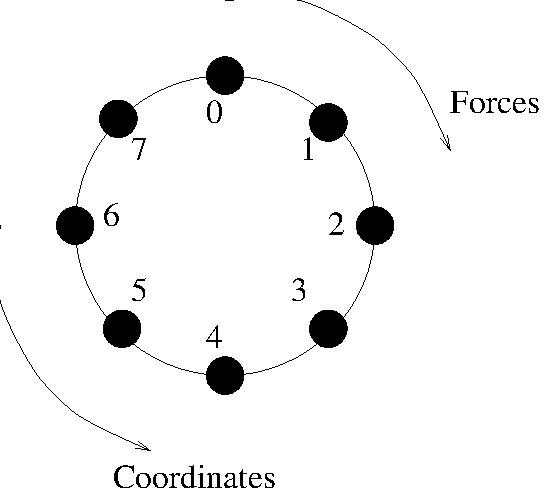
\includegraphics[width=6cm]{plots/ring}}
\caption {Data flow in a ring of processors.}
\label{fig:ring}
\end {figure}

\section{Parallel Molecular Dynamics}
In this chapter we describe some details of the \swapindex{parallel}{MD}  
algorithm used 
in {\gromacs}. This also includes some other information on neighbor searching and
a side excursion to parallel sorting.
Please note the following which we use throughout this chapter:\\
{\bf definition:} {\natom}: Number of particles, {\nproc} number of processors.\\
{\gromacs} employs two different grids: the neighbor searching grid ({\nsgrid})
and the combined charge/po\-ten\-tial grid ({\fftgrid}), as will be described below.
To maximize the confusion, 
these two grids are mapped onto a grid of processors when {\gromacs} runs on a 
parallel computer.

\subsection{Domain decomposition}
Modern parallel computers, such as an IBM SP/2 or a Cray T3E
consist of relatively small numbers of relatively fast scalar
processors (typically 8 to 256).  The communication channels that are
available in hardware on these machine are not directly visible to
the programmer; a software layer (usually \normindex{MPI}) 
hides this, and makes communication from all processors to all
others possible. In contrast, in the {\gromacs} hardware~\cite{Berendsen95a}
only communication in a ring was available, {\ie} each processor could communicate
with its direct neighbors only.

It seems logical to map the computational box of an MD simulation system 
to a 3D grid of 
processors ({\eg} 4x4x4 for a 64 processor system). This ensures that most 
interactions that are local in space can be computed with information from 
neighboring processors only. However, this means that there have to be
communication channels in 3 dimensions too, which is not necessarily the case.
Although this may be overcome in software, such a mapping complicates the MD
software as well, without clear performance benefits on most
parallel computers. 

Therefore we opt for a simple one-dimensional division scheme
for the computational box. Each processor gets a slab of this box in the 
X-dimension.
For the communication between processors this has two main advantages:
\begin{enumerate}
\item   Simplicity of coding. Communication can only be to two neighbors
        (called {\em left} and {\em right} in {\gromacs}).
\item   Communication can usually be done in large chunks, which makes it
        more efficient on most hardware platforms.
\end{enumerate}

Most interactions in molecular dynamics have in principle a
short-range character.  Bonds, angles and dihedrals are guaranteed to
have the corresponding particles close in space.


\subsection{Domain decomposition for non-bonded forces}
For large parallel computers, domain decomposition is preferable over
particle decomposition, since it is easier to do load
balancing. Without load balancing the scaling of the code is rather
poor. For this purpose, the computational box is divided in {\nproc}
slabs, where {\nproc} is equal to the number of processors. There are
multiple ways of dividing the box over processors, but since the
{\gromacs} code assumes a ring topology for the processors, it is
logical to cut the system in slabs in just one dimension, the X
dimension.  The algorithm for neighbor searching then becomes:
\begin{enumerate}
\item   Make a list of charge group indices sorted on (increasing) X coordinate
        (\figref{parsort}).
        {\bf Note} that care must be taken to parallelize the sorting algorithm
        as well. See \secref{parsort}.
\item   Divide this list into slabs, with each slab having the same number of
        charge groups
\item   Put the particles corresponding to the local slab on a 3D {\nsgrid} as 
        described in \secref{nsgrid}.
\item   Communicate the {\nsgrid} to neighboring processors (not necessarily to all
        processors). The amount of neighboring {\nsgrid} cells (N$_{gx}$) to 
        communicate is determined by the cut-off length $r_c$ according to
        \beq
        N_{gx}  ~=~     \frac{r_c \nproc}{l_x}   
        \eeq
        where $l_x$ is the box length in the slabbing direction. 
\item   On each processor compute the neighbor list for all charge groups in
        its slab using the normal grid neighbor-searching.
\end{enumerate}

\begin{figure}
\centerline{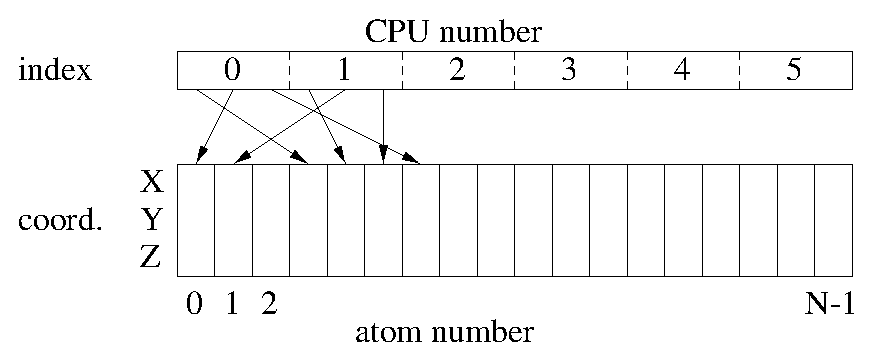
\includegraphics[width=10cm]{plots/parsort}}
\caption[Index in the coordinate array.]{Index in the coordinate
array. The division in slabs is indicated by dashed lines.}
\label{fig:parsort}
\end{figure}

For homogeneous system, this is close to an optimal load balancing,
without actually doing load balancing. For inhomogeneous system, such
as membranes or interfaces, the slabs should be perpendicular to the
interface; this way, each processor has ``a little bit of
everything''.  The {\gromacs} utility program {\tt editconf} has an
option to rotate a whole computational box.

The following observations are important here:
\begin{itemize}
\item   Particles may diffuse from one slab to the other, therefore each processor
        must hold coordinates for all particles all the time, and distribute forces
        back to all processors as well.
\item   Velocities are kept on the ``home processor'' for each particle,
        where the integration of Newton's equations is done.
\item   Fixed interaction lists (bonds, angles etc.) are kept each
        on a single processor.  Since all processors have all
        coordinates, it does not matter where interactions are
        calculated.  The division is actually done by the {\gromacs}
        preprocessor {\tt grompp} and care is taken that, as far as
        possible, every processor gets the same number of bonded
        interactions.
\end{itemize}

In all, this makes for a mixed particle decomposition/domain decomposition scheme
for parallelization of the MD code. The communication costs are four times higher
than for the simple particle decomposition method described in \secref{par}
(the whole coordinate and force array are communicated across the whole ring,
rather than half the array over half the ring).
However, for large numbers of processors the improved load balancing 
compensates this easily.

\subsection{Parallel \normindex{PPPM}}
A further reason for domain decomposition is the PPPM algorithm. This
algorithm works with a 3D Fast Fourier Transform. It employs a
discrete grid of dimensions (\nx,\ny,\nz), the {\fftgrid}. The
algorithm consist of five steps, each of which have to be
parallelized:
\begin{enumerate}
\item   Spreading charges on the {\fftgrid} to obtain the charge 
        distribution $\rho(\ve{r})$.
        This bit involves the following sub-steps:
        \begin{enumerate}
        \item[{\bf a.}] put particle in the box
        \item[{\bf b.}] find the {\fftgrid} cell in which the particle resides
        \item[{\bf c.}] add the charge of the particle times the appropriate
                        weight factor (see \secref{pppm}) to 
                        each of the 27 grid points (3 x 3 x 3).
        \end{enumerate}
        In the parallel case, the {\fftgrid} 
        must be filled on each processor with its
        share of the particles, and subsequently the {\fftgrid}s of all processors
        must be summed to find the total charge distribution. It may be clear that
        this induces a large amount of unnecessary work, unless we use domain
        decomposition. If each processor only has particles in a certain region
        of space, it only has to calculate the charge distribution for 
        that region of space. Since {\gromacs} works with slabs, this means that
        each processor fills the {\fftgrid} cells corresponding to its slab in space
        and addition of {\fftgrid}s need only be done for neighboring slabs.\\
        To be more precise, the slab $x$ for processor $i$ is defined as:
        \beq
        i\, \frac{l_x}{M} \le x <\, (i+1)\frac{l_x}{M}
        \eeq
        Particle with this $x$ coordinate range will add to the charge distribution
        on the following range of 
        of {\fftgrid} slabs in the $x$ direction:
        \beq
        {\rm trunc}\left(i\,\frac{l_x \nx}{M}\right)-1 \le i_x \le {\rm trunc}\left((i+1)\,\frac{l_x \nx}{M}\right)+2
        \eeq
        where trunc indicates the truncation of a real number to the largest integer
        smaller than or equal to that real number.
        
\item   Doing the Fourier transform of the charge distribution $\rho(\ve{r})$ 
        in parallel to obtain $\hat{\rho}(\ve{k})$. This is done using
        the FFTW library (see \href{http://www.fftw.org}{www.fftw.org})
        which employs the MPI library for message passing programs
        (note that there are also \swapindex{shared}{memory} versions
        of the FFTW code).\\
        This FFT algorithm actually use slabs as well (good
        thinking!).  Each processor does 2D FFTs on its slab, and then
        the whole {\fftgrid} is transposed {\em in place}
        ({\ie} without using extra memory).  This means that after the
        FFT the X and Y components are swapped.  To complete the FFT,
        this swapping should be undone in principle (by transposing
        back).  Happily the FFTW code has an option to omit this,
        which we use in the next step.
\item   Convolute $\hat{\rho}(\ve{k})$ with the Fourier transform of the
        charge spread function $\hat{g}(\ve{k})$ (which we have tabulated before)
        to obtain the potential $\hat{\phi}(k)$. 
        As an optimization, we store the $\hat{g}(\ve{k})$  in transposed form
        as well, matching the transposed form of $\hat{\rho}(\ve{k})$
        which we get from the FFTW routine. After this step we have the 
        potential $\hat{\phi}(k)$ in Fourier space, but still on the transposed
        {\fftgrid}.
\item   Do an inverse transform of $\hat{\phi}(k)$ to obtain
        ${\phi}(\ve{r})$. Since the algorithm must do a transpose of the data
        this step actually yields the wanted result: the un-transposed
        potential in real space.
\item   Interpolate the potential ${\phi}(\ve{r})$ in real space at the particle
        positions to obtain forces and energy. For this bit the same considerations
 	about parallelism hold as for the charge spreading. However in this
        case more neighboring grid cells are needed, implying that we need
        the following set of {\fftgrid} slabs in the $x$ direction:
        \beq
        {\rm trunc}\left(i\,\frac{l_x \nx}{M}\right)-3 \le i_x \le {\rm trunc}\left((i+1)\,\frac{l_x \nx}{M}\right)+4
        \eeq

\end{enumerate}
The algorithm as sketched above requires communication for spreading
the charges, for the forward and backward FFTs, and for interpolating
the forces.  The {\gromacs} bits of the program use only left and
right communication, {\ie} using two communication channels. The FFTW
routines actually use other forms of communication as well, and these
routines are coded with MPI routines for message passing. This implies
that {\gromacs} can only perform the PPPM algorithm on parallel
computers that support MPI. However, most
\swapindex{shared}{memory} computers, such as the SGI Origin, also
support MPI using the 
shared memory for communication.

\subsection{Parallel sorting}
\label{sec:parsort}
For the domain decomposition bit of {\gromacs} it is necessary to sort the 
coordinates (or rather the index to coordinates) every time a neighbor list is made.
If we use brute force, and sort all coordinates on each processor (which is 
technically possible since we have all the coordinates), then this sorting procedure
will take a constant wallclock time, proportional to {\natom}$^2\log${\natom}, 
regardless of the number of processors. We can however do a little
better, if we assume that particles diffuse only slowly.
A parallel sorting algorithm can be conceived as follows: \\
At the first step of the simulation
\begin{enumerate}
\item   Do a full sort of all indices using {\eg} the  Quicksort algorithm that is
        built-in in the standard C-library
\item   Divide the sorted array into slabs (as described above see 
        \figref{parsort}).
\end{enumerate}
At subsequent steps of the simulation:
\begin{enumerate}
\item   Send the indices for each processor to the preceding processor (if
        not processor 0) and to the next processor (if not {\nproc}-1). The 
        communication associated with this operation is proportional to
        2{\natom}/{\nproc}.
\item   Sort the combined indices of the three (or two) processors. Note that
        the CPU time associated with sorting is now
        (3{\natom}/{\nproc})$^2\log$ (3{\natom}/{\nproc}).
\item   On each processor, the indices belonging to its slab can be determined
        from the order of the array (\figref{parsort}).
\end{enumerate}

%\section{A Worked Example}
%Suppose our box size is 4.0 nm and the cut-off is 0.8 nm. For neighborsearching 
%we use {\dgrid} = 2, such that there 10 {\nsgrid} cells.

